% !TEX root = master.tex

We have developed techniques for automated sky analysis, bulge+disc fitting and truncation characterisation. We have compiled truncation parameters for a large sample of galaxies and investigated their correlations cluster environment. 

Figure \ref{fig: prop_hist} shows that truncated galaxies have a wider range of effective bulge magnitudes with smaller \sersic indices. This suggests that truncated galaxies have a more concentrated brighter centre consistent with the hypothesis of formation by galaxy harassment whereby the centre receives gas from the outskirts.

There is one type-II in our study, making up just under 2\% of our sample. This is consistent with the findings of \citet{erwin_strong_2012} in that there are very few if not any disks which exhibit downbending in the cluster environment. 
\begin{figure}
	\centering
	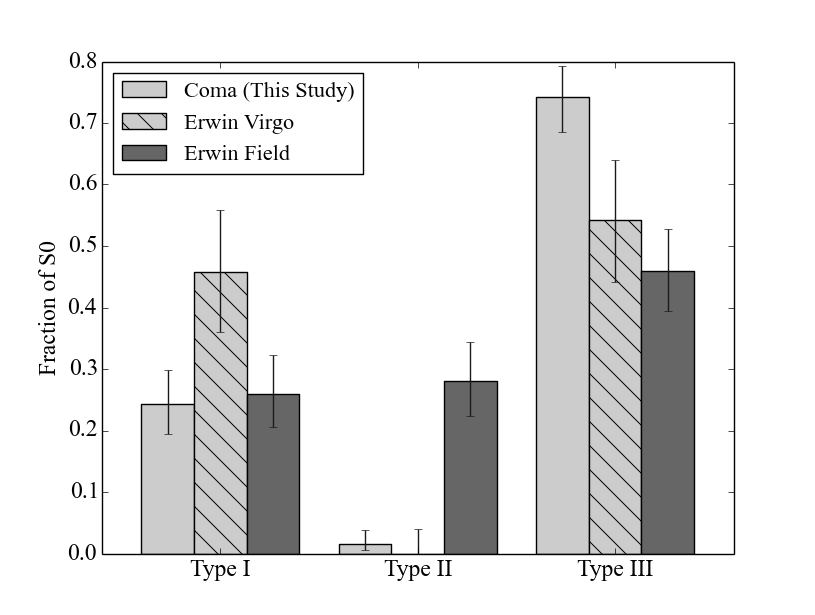
\includegraphics[width=\textwidth, scale=0.6]{figs/total_bar_chart_truncs_incl_field.png}
	\caption{Comparison of Type fraction in the Coma cluster to the Virgo Cluster and the field \citep{erwin_strong_2012}. Error bars show 68\% confidence intervals \citep{wilson_probable_1927}}
\end{figure}
However, our study finds that there is a greater divide between Type-Is and Type-IIIs with 24\% and 74\% respectively. The frequency of type-I S0s appears not to be dependent on environment. This implies that the difference between field and cluster type-II fraction is made up of type-III. This strongly suggests that type-Is form by the same path in both the field and cluster environments with the other two types forming by a different one. For this to be true requires that either type-IIs are not generated in the cluster at all, or they undergo a massive increase in outer disk brightness or simply that many more type-IIIs are created. 

The model galaxy found in \citet{moore_survival_1999,moore_galaxy_1996} was transformed from a classical type-I disk to one with a mild anti-truncation by way of galaxy harassment. Given the mildness of the upbending, it is unlikely that process can transform from type-II to type-III. The creation of type-IIs is therefore presumably suppressed at all times during cluster evolution or so slow compared to the anti-truncation that current distribution contains little downbending disks.

Given that Virgo and Coma are at roughly the same close redshift ($z=0.03, 0.02$ respectively) \citep{bower_precision_1992} and that the cluster sample in \citet{erwin_strong_2012} is under half the size of this study, it is possible that with a larger sample, Virgo may exhibit the same relation as found here.

The weak trend in figure \ref{fraction vs dist} could indicate that there is an increase in type-IIIs with decreasing cluster-centric distance, but more data is required to resolve the trend. If there is indeed a correlation between radius and frequency of type-IIIs, this would strongly suggest that their formation mechanism is galaxy interaction based. However, it is currently equally, if not more, probable that there is no trend within the cluster itself. 

\subsection{Problems with this method}
Fitting in 1D is swift and easier than a full 2D decomposition. However, neglecting most of the light of the galaxy impacts on the accuracy of the profile fitted. Any perturbation or artefact -such as a bar or flat-fielding error- included in the major axis wedge cannot be easily or safely removed. Therefore, the two major axis profiles will strongly disagree if there is a slight difference between them. Further problems arise from the combination of profiles from different cameras. 

Combining four bootstraps is effective when the individual results are already close to each other (within $\sim 1\sigma$) and a disagreeing fourth may be discarded provided the other three agree. When there is a divide in parameter space larger than $\sim 2\sigma$ the resulting combination will yield a result which neither bootstrap group supports and with large errors. 

Sky detection has worked effectively in this investigation but whether our values are correct or not is untestable until there are more readings around the galaxy in addition to those at the end of the major-axis. 